% Using Free and Open Source Solutions in Geospatial Science Education
% This work by Vaclav Petras is licensed under
% a Creative Commons Attribution-ShareAlike 4.0 International License.

% Session
%
% NS52A: A Tour of Open-Source Software Packages for the Geosciences II
%
% This session will be a rapid-fire tour of open source tools freely available for
% researchers in the geosciences. The fast-growing open-source software ecosystem
% is creating new tools and changing paradigms for how computers and
% collaborations are used to study Earth processes. If you have written
% open-source software that could be useful to others, we look forward to seeing
% your submission. This session will not only be an opportunity to showcase your
% own packages and learn about other available tools, we also hope it will be an
% opportunity to connect with others working on related problems and lead to new
% collaborations. The session will be accompanied by posters where the audience
% can engage individually with the presenters.
%
% Abstract
%
% GRASS GIS (grass.osgeo.org) is an open source software for geospatial analysis,
% remote sensing, general geoprocessing and visualization. It is a
% community-driven project with over 35 years of continuous software development
% based on scientific expertise from many geospatial fields. It is characterized
% by long-term releases, stable APIs, and emphasis on science. GRASS GIS
% distribution strives to provide single integrated environment for 2D and 3D
% raster analysis, image processing, vector data analysis, and spatio-temporal
% data processing. It supports large raster files (billions of cells), vector
% topology, coupling with databases, and 64 bit memory. New code based on recent
% research is typically contributed to GRASS GIS Addons repository. Mature, widely
% used code is then moved to the main code base to maximize integration and
% availability. Whether it is addons or the main code base, code is usually
% maintained by the community and preserved in long term even in cases when the
% original author no longer supports the code. To support the needs of scientists,
% the documentation includes not only links to the source code, its history, and
% its authors, but also links to research papers that describe the algorithms
% implemented in the modules.
%
% Code is not only maintained but also extended and improved. For example,
% watershed and stream extraction using least cost path approach was implemented
% in 1989 and extended for massive datasets in 2011. Similarly, vector topology
% cleaning was introduced in 2002, updated over time and substantially improved in
% 2016. Another example is a solar energy module available since 1993 and
% parallelized in 2017. The current stable version of GRASS GIS 7.4 provides new
% features for geosciences such as temporal framework with temporal algebra for
% large time-series processing, fusion of elevation models from various sensors,
% 3D flows, landform detection, image segmentation, simplified batch processing,
% and integrated Python editor among others. GRASS GIS runs in various
% environments including Linux, Mac, Windows, Docker, Raspberry Pi, and on HPC
% clusters. The modules are written in Python, C, or C++. Besides command line
% interface, GRASS GIS provides a graphical user interface, a Python API, and a C
% API. Interfaces with other languages such as R and Ruby are supplied by
% collaborating communities.

\documentclass[xcolor={dvipsnames,usenames},beamer,aspectratio=169]{beamer}
% ,handout,notes=show

\makeatletter
\def\beamer@framenotesbegin{% at beginning of slide
  \gdef\beamer@noteitems{}%
  \gdef\beamer@notes{{}}% used to be totally empty.
}
\makeatother

\usepackage{textcomp}
\usepackage[utf8]{inputenc}
\usepackage[american]{babel}
\usepackage{graphicx}
\usepackage{url}
\usepackage{amssymb}

\usepackage{alltt}

\usepackage{tikz}
\usetikzlibrary{arrows,shapes,spy,calc}

\tikzstyle{every picture}+=[remember picture]
\tikzstyle{na} = [baseline=-.5ex]

% don't count bacup slides
\newcommand{\backupbegin}{
   \newcounter{finalframe}
   \setcounter{finalframe}{\value{framenumber}}
}
\newcommand{\backupend}{
   \setcounter{framenumber}{\value{finalframe}}
}

% frames have to be fragile
\newif\ifnotes
% % \notestrue

% \notestrue


\ifnotes
\setbeamertemplate{note page}[plain]
% \setbeamertemplate{note page}[compress]
\setbeamerfont{note page}{size=\large}
% \setbeameroption{show only notes}
\setbeameroption{show notes}
\usepackage{pgfpages}
\pgfpagesuselayout{2 on 1}[a4paper,border shrink=5mm]%
\else
%\setbeameroption{hide notes}
\fi
%\notesfalse

\usepackage[absolute,overlay]{textpos}

\usepackage{listings}

% Fira Sans, GRASS GIS branding sans serif font
\usepackage{FiraSans}
\renewcommand*\oldstylenums[1]{{\firaoldstyle #1}}

% \usetheme{Warsaw}
\usetheme{Madrid}
% \usetheme{Frankfurt}
% \useoutertheme{infolines}
\definecolor{GRASSGISGreen}{HTML}{009000}
\usecolortheme[named=GRASSGISGreen]{structure}
\setbeamertemplate{navigation symbols}{}

\setbeamertemplate{itemize items}[default]
\setbeamertemplate{enumerate items}[default]
% \useinnertheme{rectangles}
\setbeamertemplate{blocks}[default]


%%%%%%%%%%%%%%%%%%%%%%%%%%%%%%%%%%%%%%%%%%%%%%%%%%%%%%%%%%%%%%%%%%%%
%%%%%%%%%%%%%%%%%%%%%%%%%%%%%%%%%%%%%%%%%%%%%%%%%%%%%%%%%%%%%%%%%%%%

% \newcommand{\n}[1]{$^{\color{gray}{\mbox{\tiny#1}}}$}
\newcommand{\n}[1]{$^{\textcolor{gray}{\mbox{\tiny #1}}}$}

%%%%%%%%%%%%%%%%%%%%%%%%%%%%%%%%%%%%%%%%%%%%%%%%%%%%%%%%%%%%%%%%%%%%%%%%%%%%%%%
\newcommand{\gmodule}[1]{\href{http://grass.osgeo.org/grass74/manuals/#1.html}{\emph{#1}}}
\newcommand{\amodule}[1]{\href{http://grass.osgeo.org/grass74/manuals/addons/#1.html}{\emph{#1}}}
\newcommand{\module}[1]{\emph{#1}}
\newcommand{\grasslink}{\href{http://grass.osgeo.org/}{GRASS GIS}}

%%%%%%%%%%%%%%%%%%%%%%%%%%%%%%%%%%%%%%%%%%%%%%%%%%%%%%%%%%%%%%%%%%%%
%%%%%%%%%%%%%%%%%%%%%%%%%%%%%%%%%%%%%%%%%%%%%%%%%%%%%%%%%%%%%%%%%%%%

\title[GRASS GIS]{\textbf{GRASS}\,{\firalight GIS}: A General-purpose Geospatial Research Tool}
\subtitle{
AGU 2018 Fall Meeting
\\
\scriptsize
NS52A: A Tour of Open-Source Software Packages for the Geosciences II
}
%\pdforstring{}{}

\newcommand{\inst}[1]{\hspace{2pt}$^{\mbox{\normalsize#1}}$\hspace{-7pt}}
\newcommand{\instlist}[1]{\hspace{1pt}$^{\mbox{#1}}$\hspace{2pt}}

\author[Vaclav Petras]{
Helena Mitasova\inst{1},
Vaclav Petras\inst{1}\,*\hspace{-7pt},
Anna Petrasova\inst{1},
\&
Markus Neteler\hspace{0.05em}\inst{2}
\\
Scientific Team: GRASS GIS Development Team**
}

\institute[NC State University]
{%
\instlist{1}Center for Geospatial Analytics, NCSU, USA;
\instlist{2}mundialis, Germany
\\
*\texttt{wenzeslaus@gmail.com, vpetras@ncsu.edu, @vaclavpetras}
\\
% using Black Duck Open Hub to ``guestimate'' that
**Includes over 10 other members of the core team and numerous other contributors

\bigskip

\includegraphics[height=0.04\textwidth]{ncstate}%
~

\includegraphics[height=0.06\textwidth]{mundialis}%
}

\date{December 14, 2018}

\setbeamercovered{transparent}

\hypersetup{%
 pdfauthor={Vaclav Petras},%
 pdfsubject={Point clouds and GRASS GIS talk at ISPRS 2016},%
 pdfkeywords={3D rasters} {decimation} {sampling} {binning}
   {LAS} {PDAL} {PCL} {Kinect}
   {v.in.lidar} {r.in.lidar} {r.in.kinect} {libLAS}
   {geospatial modeling}
   {free software} {open source} {open science}
}

\usepackage{tipa}
\newcommand{\pron}[2]{#1 [#2]}


%%%%%%%%%%%%%%%%%%%%%%%%%%%%%%%%%%%%%%%%%%%%%%%%%%%%%%%%%%%%%%%%%%%%
% when images are placed in these directories, we don't have to specify the directory
% just the filename
\graphicspath{{logos/}{images/}}


%%%%%%%%%%%%%%%%%%%%%%%%%%%%%%%%%%%%%%%%%%%%%%%%%%%%%%%%%%%%%%%%%%%%
%%%%%%%%%%%%%%%%%%%%%%%%%%%%%%%%%%%%%%%%%%%%%%%%%%%%%%%%%%%%%%%%%%%%
%%%%%%%%%%%%%%%%%%%%%%%%%%%%%%%%%%%%%%%%%%%%%%%%%%%%%%%%%%%%%%%%%%%%
%%%%%%%%%%%%%%%%%%%%%%%%%%%%%%%%%%%%%%%%%%%%%%%%%%%%%%%%%%%%%%%%%%%%
\begin{document}

\newcommand{\logowidth}{1.0em}
\newcommand{\logospace}{\hspace{0.2em}}
\newcommand{\includecclogo}[1]{\includegraphics[width=\logowidth]{#1}}

%%%%%%%%%%%%%%%%%%%%%%%%%%%%%%%%%%%%%%%%%%%%%%%%%%%%%%%%%%%%%%%%%%%%
\frame{
\titlepage
\begin{center}
\vspace{-3ex}
\href{http://creativecommons.org/licenses/by-sa/4.0/}{
\includecclogo{cc}
\logospace
\includecclogo{by}
\logospace
\includecclogo{sa}
}
\end{center}
}


%%%%%%%%%%%%%%%%%%%%%%%%%%%%%%%%%%%%%%%%%%%%%%%%%%%%%%%%%%%%%%%%%%%%%
\begin{frame}{GRASS GIS}

\begin{columns}
\begin{column}{0.6\textwidth}

\begin{itemize}
  \item all in one
  \begin{itemize}
   \item hydrology modeling, image segmentation, point clustering, \ldots
  \end{itemize}
  \item driven by needs of users
  \begin{itemize}
   \item Community-driven project direct access to development process
  \end{itemize}
  \item from small laptops to supercomputers
  \begin{itemize}
   \item Raspberry Pi, Windows, Mac, GNU/Linux, FreeBSD, IBM~AIX
  \end{itemize}
  \item learn now, use forever
  \begin{itemize}
    \item over 35 years of development and interface refinement
  \end{itemize}
\end{itemize}

\end{column}
\begin{column}{0.3\textwidth}

\begin{center}
  
\includegraphics[width=\textwidth]{logos/grass_gis}
\end{center}

\vspace*{-1ex}

\textcolor{gray}{
\footnotesize
latest release 7.4.3
\scriptsize
(Nov 26, 2018)
}

\end{column}
\end{columns}

\end{frame}


%%%%%%%%%%%%%%%%%%%%%%%%%%%%%%%%%%%%%%%%%%%%%%%%%%%%%%%%%%%%%%%%%%%%%
\begin{frame}{Novel methods are included}

\begin{columns}
\begin{column}{0.6\textwidth}

\begin{itemize}
  \item r.sim.water (Mitas and Mitasova, 1998) overland flow simulation
  \item Least cost flow r.watershed from ’89
\end{itemize}

\end{column}
\begin{column}{0.3\textwidth}

\begin{center}
  
\includegraphics[width=\textwidth]{logos/grass_gis}
\end{center}

\vspace*{-1ex}

\textcolor{gray}{
\footnotesize
latest release 7.4.3
\scriptsize
(Nov 26, 2018)
}

\end{column}
\end{columns}

\end{frame}


%%%%%%%%%%%%%%%%%%%%%%%%%%%%%%%%%%%%%%%%%%%%%%%%%%%%%%%%%%%%%%%%%%%%%
\begin{frame}{Innovations are preserved}

\begin{columns}
\begin{column}{0.6\textwidth}

\begin{itemize}
  \item r.sim.water (Mitas and Mitasova, 1998) overland flow simulation
  \item Least cost flow r.watershed from ’89
\end{itemize}

\end{column}
\begin{column}{0.3\textwidth}

\begin{center}
  
\includegraphics[width=\textwidth]{logos/grass_gis}
\end{center}

\vspace*{-1ex}

\textcolor{gray}{
\footnotesize
latest release 7.4.3
\scriptsize
(Nov 26, 2018)
}

\end{column}
\end{columns}

\end{frame}


%%%%%%%%%%%%%%%%%%%%%%%%%%%%%%%%%%%%%%%%%%%%%%%%%%%%%%%%%%%%%%%%%%%%%
\begin{frame}{Code is further developed}

\begin{columns}
\begin{column}{0.6\textwidth}

\begin{itemize}
  \item v.outlier module serves as a base for v.lidar.mcc implementing Multiscale Curvature Classification.
  \item v.surf.rst for spatial interpolation developed in ’90s; improved several times and parallelized for version 7.4.
\end{itemize}

\end{column}
\begin{column}{0.3\textwidth}

\begin{center}
  
\includegraphics[width=\textwidth]{logos/grass_gis}
\end{center}

\vspace*{-1ex}

\textcolor{gray}{
\footnotesize
latest release 7.4.3
\scriptsize
(Nov 26, 2018)
}

\end{column}
\end{columns}

\end{frame}

%%%%%%%%%%%%%%%%%%%%%%%%%%%%%%%%%%%%%%%%%%%%%%%%%%%%%%%%%%%%%%%%%%%%%
\begin{frame}{Tools used by other scientists}

\begin{columns}
\begin{column}{0.6\textwidth}

\begin{itemize}
  \item v.outlier module serves as a base for v.lidar.mcc implementing Multiscale Curvature Classification.
  \item v.surf.rst for spatial interpolation developed in ’90s; improved several times and parallelized for version 7.4.
\end{itemize}

\end{column}
\begin{column}{0.3\textwidth}

\begin{center}
  
\includegraphics[width=\textwidth]{logos/grass_gis}
\end{center}

\vspace*{-1ex}

\textcolor{gray}{
\footnotesize
latest release 7.4.3
\scriptsize
(Nov 26, 2018)
}

\end{column}
\end{columns}

\end{frame}

%%%%%%%%%%%%%%%%%%%%%%%%%%%%%%%%%%%%%%%%%%%%%%%%%%%%%%%%%%%%%%%%%%%%%
\begin{frame}{Published algorithms are implemented}

\begin{columns}
\begin{column}{0.6\textwidth}

\begin{itemize}
  \item v.outlier module serves as a base for v.lidar.mcc implementing Multiscale Curvature Classification.
  \item v.surf.rst for spatial interpolation developed in ’90s; improved several times and parallelized for version 7.4.
\end{itemize}

\end{column}
\begin{column}{0.3\textwidth}

\begin{center}
  
\includegraphics[width=\textwidth]{logos/grass_gis}
\end{center}

\vspace*{-1ex}

\textcolor{gray}{
\footnotesize
latest release 7.4.3
\scriptsize
(Nov 26, 2018)
}

\end{column}
\end{columns}

\end{frame}


%%%%%%%%%%%%%%%%%%%%%%%%%%%%%%%%%%%%%%%%%%%%%%%%%%%%%%%%%%%%%%%%%%%%%
\begin{frame}{Publishing code}

\begin{block}{}
 \begin{itemize}
  \item Ask for access to GRASS GIS Addons at
        \\
        \href{https://grass.osgeo.org/development/code-submission/}{\texttt{grass.osgeo.org/development/code-submission}}
  \item Example GRASS GIS module
        \\
        \href{https://gitlab.com/vpetras/r.example.plus/}{\texttt{gitlab.com/vpetras/r.example.plus}}
 \end{itemize}
\end{block}

\bigskip
\centering

\begin{tabular}{clc}
\begin{minipage}{0.16\textwidth}

\includegraphics[width=\textwidth]{grass_gis}
\end{minipage}
&
\begin{minipage}{0.5\textwidth}
\footnotesize
\href{https://grass.osgeo.org}{%
Get GRASS GIS at\\
\texttt{grass.osgeo.org}%
}

\bigskip

{
\footnotesize
\href{https://lists.osgeo.org/listinfo/grass-user}{GRASS user mailing list}\\
\href{https://lists.osgeo.org/listinfo/grass-user}{\texttt{lists.osgeo.org/listinfo/grass-user}}
}

\bigskip

{
\footnotesize
Source files for poster and slides available at\\
\href{https://trac.osgeo.org/grass/browser/grass-promo/}%
  {\texttt{trac.osgeo.org/grass/browser/grass-promo}}
}
\end{minipage}
&
\begin{minipage}{0.2\textwidth}
% \includegraphics[width=\textwidth]{talks_qr}
\end{minipage}
\end{tabular}

\end{frame}

% don't count the backup and ack slides
\backupbegin

%%%%%%%%%%%%%%%%%%%%%%%%%%%%%%%%%%%%%%%%%%%%%%%%%%%%%%%%%%%%%%%%%%%%%
\begin{frame}{Providing algorithms to the community}

\begin{itemize}
  \item new landform recognition approach -- geomorphons
\end{itemize}

\begin{columns}
\begin{column}{0.4\textwidth}

\begin{itemize}
  % Adam Mickiewicz University and University of Cincinnati
  \item by Jasiewicz and Stepinski
    {\tiny from AMU, Poland and University of Cincinnati, USA}
  \item not just a paper
    {\tiny Geomorphology, 2013}
  \item not just a code
    \\{\tiny at some webpage}
  \item \amodule{r.geomorphon}
    \\{\tiny module in GRASS GIS addons repository}
\end{itemize}

\end{column}
\begin{column}{0.58\textwidth}

\begin{center}
%   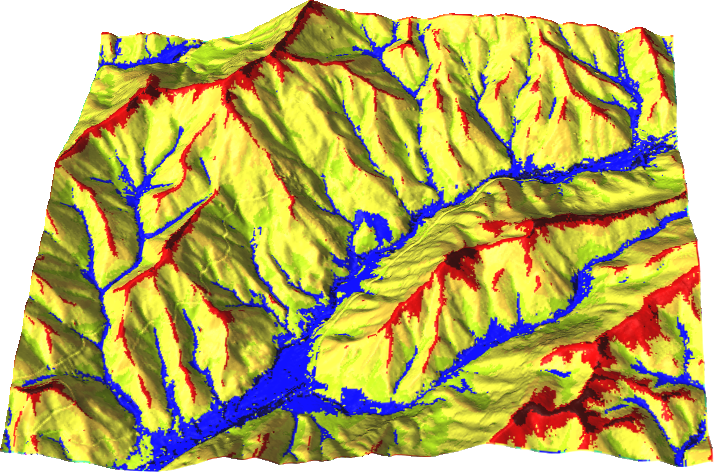
\includegraphics[width=\textwidth]{vis/geomorphon_3d}
\end{center}

\end{column}
\end{columns}

\end{frame}


%%%%%%%%%%%%%%%%%%%%%%%%%%%%%%%%%%%%%%%%%%%%%%%%%%%%%%%%%%%%%%%%%%%%%
\begin{frame}{GRASS GIS}

\begin{columns}
\begin{column}{0.6\textwidth}

\begin{itemize}
  \item all in one
  \begin{itemize}
   \item hydrology modeling, image segmentation, point clustering, \ldots
  \end{itemize}
  \item driven by needs of users
  \begin{itemize}
   \item direct access to development process
  \end{itemize}
  \item from small laptops to supercomputers
  \begin{itemize}
   \item Raspberry Pi, Windows, Mac, GNU/Linux, FreeBSD, IBM~AIX
  \end{itemize}
  \item learn now, use forever
  \begin{itemize}
    \item over 30 years of development and interface refinement
  \end{itemize}
  \item used by
  \begin{itemize}
    \item US Oak Ridge National Laboratory, Edmund Mach Foundation, JRC, \ldots
  \end{itemize}
\end{itemize}

\end{column}
\begin{column}{0.3\textwidth}

\begin{center}
  
\includegraphics[width=\textwidth]{logos/grass_gis}
\end{center}

\textcolor{gray}{
\footnotesize
latest release 7.0.4 \\May~1,~2016
}

\end{column}
\end{columns}

\end{frame}


%%%%%%%%%%%%%%%%%%%%%%%%%%%%%%%%%%%%%%%%%%%%%%%%%%%%%%%%%%%%%%%%%%%%%
\begin{frame}{GUI}

\begin{center}
%   \includegraphics[width=0.9\textwidth]{grass/r_in_lidar_gui}
\end{center}

\end{frame}


%%%%%%%%%%%%%%%%%%%%%%%%%%%%%%%%%%%%%%%%%%%%%%%%%%%%%%%%%%%%%%%%%%%%%
\begin{frame}{Python and command line interfaces}

\definecolor{mod}{RGB}{7,96,143}
\definecolor{opt}{RGB}{239,84,18}
\definecolor{flg}{RGB}{239,84,18}
\definecolor{txt}{RGB}{45,146,45}
\definecolor{bash}{RGB}{200,200,200}
\definecolor{import}{RGB}{200,200,200}

\Large

Command Line:

\LARGE

\begin{alltt}
\textcolor{mod}{r.in.lidar} \textcolor{opt}{input}=\textcolor{txt}{points.las} \textcolor{bash}{\char`\\}
\\%
\newlength{\shindent}
\settowidth{\shindent}{r.in.lidar~}
\rule{\shindent}{0pt}%
\textcolor{opt}{output}=\textcolor{txt}{elevation} -\textcolor{flg}{e}
\end{alltt}

\Large

Python:

% \char`_ is to get same underscore as in \verb

\LARGE

\begin{alltt}
\textcolor{import}{from grass.script import run\char`_command}
\\
run\char`_command('\textcolor{mod}{r.in.lidar}',
%
\newlength{\pyindent}%
\settowidth{\pyindent}{run\_command(}%
\\%
\rule{\pyindent}{0pt}\,%
\textcolor{opt}{input}="\textcolor{txt}{points.las}",
\\%
\rule{\pyindent}{0pt}\,%
\textcolor{opt}{output}="\textcolor{txt}{elevation}",
\\%
\rule{\pyindent}{0pt}\,%
flags='\textcolor{flg}{e}')
\end{alltt}

\end{frame}


%%%%%%%%%%%%%%%%%%%%%%%%%%%%%%%%%%%%%%%%%%%%%%%%%%%%%%%%%%%%%%%%%%%%%
\begin{frame}{Graphical Modeler}

\begin{center}
%   \includegraphics[width=0.9\textwidth]{grass/modeler}
\end{center}

\end{frame}


%%%%%%%%%%%%%%%%%%%%%%%%%%%%%%%%%%%%%%%%%%%%%%%%%%%%%%%%%%%%%%%%%%%%%
\begin{frame}{Using other open source projects}

\begin{columns}
\begin{column}{0.5\textwidth}

\begin{block}{\module{r.in.kinect}}
 \begin{itemize}
  \item scans using Kinect
  \item OpenKinect libfreenect2
  \item Point Cloud Library (PCL)
  \item GRASS GIS libraries
 \end{itemize}
\end{block}

% inner columns
\begin{columns}
\begin{column}{0.6\textwidth}
\small

used in Tangible~Landscape

\end{column}
\begin{column}{0.2\textwidth}

% \includegraphics[width=\textwidth]{logos/tangible_landscape}

\end{column}
\end{columns}
% end of inner columns

\end{column}
\begin{column}{0.45\textwidth}

\begin{center}
%   \includegraphics[width=\textwidth]{tangible/face}
\end{center}

\end{column}
\end{columns}

\end{frame}


%%%%%%%%%%%%%%%%%%%%%%%%%%%%%%%%%%%%%%%%%%%%%%%%%%%%%%%%%%%%%%%%%%%%%
\begin{frame}{Acknowledgements}

\footnotesize

\begin{columns}
\begin{column}{0.6\textwidth}

\begin{block}{Software}
The GRASS GIS Development Team, contributors, users, ...
\end{block}

\begin{block}{Datasets}

% \smallskip

Nantahala NF, NC: Forest Leaf Structure, Terrain and Hydrophysiology.
% Lidar data acquisition and processing completed
% by the National Center for Airborne Laser Mapping (\href{http://www.ncalm.org}{NCALM}).
% NCALM funding provided by NSF's Division of Earth Sciences, Instrumentation and Facilities Program.
% EAR-1043051.
Obtained from \href{http://www.opentopography.org/}{OpenTopography}.
\url{http://dx.doi.org/10.5069/G9HT2M76}
\end{block}

\begin{block}{Presentation software}
Slides were created in \textrm{\LaTeX{}} using the~\textrm{\textsc{beamer} \textit{class}}.
% all lowercase, sc and it taken from the beamer user guide
\end{block}


\end{column}
\begin{column}{0.3\textwidth}

\begin{center}
  
\includegraphics[width=\textwidth]{logos/grass_gis}
\end{center}

\end{column}
\end{columns}

\end{frame}

\backupend

\end{document}
